\documentclass[aspectratio=169,10pt]{beamer}

\usepackage{fontspec}
\setsansfont{Arial}
\setmonofont{Menlo}[Scale=0.85]
\usepackage[english,vietnamese]{babel}
\usepackage{booktabs}
\usepackage{graphicx}
\usepackage{amsmath}
\usepackage{tikz}
\usetikzlibrary{arrows.meta,positioning}

% ============================================================
%  meta.tex — shared metadata for the report (main.tex) and slides (slides/slides.tex)
%  Edit here only; both documents \input this file.
% ============================================================
\newcommand{\metaUniversity}{Đại học Bách khoa Hà Nội}
\newcommand{\metaSchool}{Trường Công nghệ Thông tin và Truyền thông}
\newcommand{\metaCourse}{Seminar 1}
\newcommand{\metaTopicCode}{A1}
\newcommand{\metaTitle}{Dùng AI phát hiện mơ hồ, thiếu sót, mâu thuẫn trong tài liệu đặc tả yêu cầu}
\newcommand{\metaShortTitle}{A1 -- AI phát hiện lỗi đặc tả yêu cầu}
\newcommand{\metaLecturer}{TS. Nguyễn Thanh Hùng}
\newcommand{\metaLecturerUnit}{Khoa Khoa học Máy tính}
\newcommand{\metaGroup}{Nhóm 4}
\newcommand{\metaSemester}{Học kỳ 20252 --- Năm học 2025--2026}
\newcommand{\metaDate}{\today}

% Members table body (ID & Name & Role)
\newcommand{\metaMembers}{%
  20251175M & Nguyễn Tùng Dương & Nhóm trưởng \\
  20251177M & Trần Xuân Nam     & Thành viên \\
  20252636M & Phạm Gia Khánh    & Thành viên \\
}
% Short author line for slide footer / title
\newcommand{\metaAuthorsShort}{Nguyễn Tùng Dương, Trần Xuân Nam, Phạm Gia Khánh}

% Generated by script/export_numbers.py -- do not edit by hand.
\newcommand{\numAIRevBorder}{4}
\newcommand{\numAIRevExpN}{5}
\newcommand{\numAIRevExpReal}{4}
\newcommand{\numAIRevN}{25}
\newcommand{\numAIRevNonReq}{4}
\newcommand{\numAIRevNot}{12}
\newcommand{\numAIRevOverLiteral}{8}
\newcommand{\numAIRevReal}{9}
\newcommand{\numAIRevRealHi}{52}
\newcommand{\numAIRevRealLo}{36}
\newcommand{\numAgyMTokens}{1{,}85}
\newcommand{\numAgyMinutes}{123}
\newcommand{\numDurTfour}{206}
\newcommand{\numDurTone}{91}
\newcommand{\numDurTthree}{211}
\newcommand{\numDurTtwo}{110}
\newcommand{\numEffortTfour}{2{,}5}
\newcommand{\numEffortTone}{4{,}0}
\newcommand{\numEffortTthree}{3{,}5}
\newcommand{\numEffortTtwo}{2{,}7}
\newcommand{\numEffortTzero}{2{,}5}
\newcommand{\numFAllTfour}{67{,}0}
\newcommand{\numFAllTone}{50{,}8}
\newcommand{\numFAllTthree}{55{,}3}
\newcommand{\numFAllTtwo}{63{,}8}
\newcommand{\numFAllTzero}{48{,}7}
\newcommand{\numFAmbTfour}{62}
\newcommand{\numFAmbTone}{37}
\newcommand{\numFAmbTthree}{42}
\newcommand{\numFAmbTtwo}{59}
\newcommand{\numFAmbTzero}{67}
\newcommand{\numFConTfour}{76}
\newcommand{\numFConTone}{79}
\newcommand{\numFConTthree}{69}
\newcommand{\numFConTtwo}{89}
\newcommand{\numFConTzero}{62}
\newcommand{\numFFlagAll}{27{,}9}
\newcommand{\numFIncTfour}{46}
\newcommand{\numFIncTone}{37}
\newcommand{\numFIncTthree}{39}
\newcommand{\numFIncTtwo}{41}
\newcommand{\numFIncTzero}{23}
\newcommand{\numFLenTfour}{69{,}7}
\newcommand{\numFLenTone}{64{,}2}
\newcommand{\numFLenTthree}{65{,}2}
\newcommand{\numFLenTtwo}{69{,}4}
\newcommand{\numFLenTzero}{52{,}0}
\newcommand{\numFSeedTfour}{100{,}0}
\newcommand{\numFSeedTone}{96{,}1}
\newcommand{\numFSeedTthree}{100{,}0}
\newcommand{\numFSeedTtwo}{97{,}8}
\newcommand{\numFSeedTzero}{65{,}3}
\newcommand{\numFTfour}{55{,}6}
\newcommand{\numFTone}{40{,}3}
\newcommand{\numFTthree}{43{,}9}
\newcommand{\numFTtwo}{52{,}8}
\newcommand{\numFTzero}{41{,}1}
\newcommand{\numFhiTfour}{63{,}2}
\newcommand{\numFhiTone}{47{,}0}
\newcommand{\numFhiTthree}{50{,}9}
\newcommand{\numFhiTtwo}{60{,}1}
\newcommand{\numFhiTzero}{51{,}9}
\newcommand{\numFleissTfour}{0{,}89}
\newcommand{\numFleissTone}{0{,}89}
\newcommand{\numFleissTthree}{0{,}77}
\newcommand{\numFleissTtwo}{0{,}83}
\newcommand{\numFloTfour}{47{,}0}
\newcommand{\numFloTone}{33{,}2}
\newcommand{\numFloTthree}{36{,}4}
\newcommand{\numFloTtwo}{45{,}0}
\newcommand{\numFloTzero}{29{,}7}
\newcommand{\numFoundTfour}{122}
\newcommand{\numFoundTone}{206}
\newcommand{\numFoundTthree}{185}
\newcommand{\numFoundTtwo}{135}
\newcommand{\numFsdTfour}{1{,}0}
\newcommand{\numFsdTone}{1{,}3}
\newcommand{\numFsdTthree}{4{,}1}
\newcommand{\numFsdTtwo}{2{,}2}
\newcommand{\numFsdTzero}{0{,}0}
\newcommand{\numGTPure}{52}
\newcommand{\numHCSlideA}{\textbf{[Đang chờ kết quả kiểm tra bởi người]}}
\newcommand{\numHCSlideB}{\textbf{[Đang chờ kết quả kiểm tra bởi người]}}
\newcommand{\numHCSlideC}{\textbf{[Đang chờ kết quả kiểm tra bởi người]}}
\newcommand{\numHumanCheckDone}{0}
\newcommand{\numJacTfour}{0{,}87}
\newcommand{\numJacTone}{0{,}93}
\newcommand{\numJacTthree}{0{,}82}
\newcommand{\numJacTtwo}{0{,}83}
\newcommand{\numLeakMaxShift}{3{,}9}
\newcommand{\numMissTfour}{7{,}1}
\newcommand{\numMissTone}{0{,}0}
\newcommand{\numMissTthree}{0{,}6}
\newcommand{\numMissTtwo}{5{,}1}
\newcommand{\numMissTzero}{57{,}7}
\newcommand{\numModelDFPlain}{3{,}7}
\newcommand{\numModelDFSkill}{2{,}8}
\newcommand{\numModelHiPlain}{5{,}3}
\newcommand{\numModelHiSkill}{5{,}3}
\newcommand{\numModelLoPlain}{2{,}2}
\newcommand{\numModelLoSkill}{0{,}1}
\newcommand{\numPFlagAll}{16{,}2}
\newcommand{\numPTfour}{39{,}7}
\newcommand{\numPTone}{25{,}2}
\newcommand{\numPTthree}{28{,}3}
\newcommand{\numPTtwo}{36{,}6}
\newcommand{\numPTzero}{40{,}0}
\newcommand{\numRAmbTfour}{92}
\newcommand{\numRAmbTone}{100}
\newcommand{\numRAmbTthree}{100}
\newcommand{\numRAmbTtwo}{94}
\newcommand{\numRAmbTzero}{52}
\newcommand{\numRConTfour}{100}
\newcommand{\numRConTone}{100}
\newcommand{\numRConTthree}{100}
\newcommand{\numRConTtwo}{100}
\newcommand{\numRConTzero}{44}
\newcommand{\numRIncTfour}{91}
\newcommand{\numRIncTone}{100}
\newcommand{\numRIncTthree}{98}
\newcommand{\numRIncTtwo}{94}
\newcommand{\numRIncTzero}{32}
\newcommand{\numRTfour}{92{,}9}
\newcommand{\numRTone}{100{,}0}
\newcommand{\numRTthree}{99{,}4}
\newcommand{\numRTtwo}{94{,}9}
\newcommand{\numRTzero}{42{,}3}
\newcommand{\numSDMaxShift}{1{,}7}
\newcommand{\numSkillDFHydro}{12{,}5}
\newcommand{\numSkillDFNeon}{11{,}6}
\newcommand{\numSkillDPHydro}{11{,}4}
\newcommand{\numSkillDPNeon}{11{,}4}
\newcommand{\numSkillDRHydro}{5{,}1}
\newcommand{\numSkillDRNeon}{6{,}4}
\newcommand{\numSkillHiHydro}{16{,}3}
\newcommand{\numSkillHiNeon}{15{,}4}
\newcommand{\numSkillLoHydro}{8{,}8}
\newcommand{\numSkillLoNeon}{7{,}8}
\newcommand{\numTokTfour}{40{,}8}
\newcommand{\numTokTone}{34{,}9}
\newcommand{\numTokTthree}{40{,}3}
\newcommand{\numTokTtwo}{38{,}2}

\graphicspath{{../report/figures/}{./}}
\usetheme{HUST}

\begin{document}

% --- Slide 1: Title ---
\begin{frame}[plain]
  \titlepage
  \note{[Dương] Kính chào thầy và các bạn. Em là Nguyễn Tùng Dương, đại diện Nhóm 4, cùng hai bạn Trần Xuân Nam và Phạm Gia Khánh. Hôm nay nhóm trình bày đề tài A1: dùng AI để phát hiện lỗi mơ hồ, thiếu sót và mâu thuẫn trong tài liệu đặc tả yêu cầu phần mềm, và đo xem AI làm tốt đến đâu so với đánh giá của chuyên gia.}
\end{frame}

% --- Slide 2: Agenda ---
\begin{frame}{Nội dung trình bày}
  \begin{enumerate}
    \item \textbf{Đặt vấn đề \& Bài toán A1:} Tầm quan trọng của chất lượng SRS và 4 câu hỏi nghiên cứu (RQ1--RQ4)
    \item \textbf{Phân loại lỗi \& Dữ liệu:} 15 tiểu loại lỗi, bộ dữ liệu PURE (107) + \texttt{seeded\_lms} (40)
    \item \textbf{Phương pháp thực nghiệm:} Bộ công cụ T0--T4, kỹ năng \texttt{SKILL.md}, chuẩn chuyên gia \& độ đo
    \item \textbf{Kết quả \& Phân tích lỗi:} Độ chính xác, tác động kỹ năng, loại lỗi khó nhất, độ ổn định
    \item \textbf{Hạn chế \& Kết luận:} Threats to validity, hướng phát triển và hỏi đáp
  \end{enumerate}
  \note{[Dương] Bài trình bày gồm năm phần. Đầu tiên là vì sao bài toán quan trọng và câu hỏi nghiên cứu. Bạn Nam sẽ trình bày cách phân loại lỗi, dữ liệu và phương pháp. Bạn Khánh trình bày cách xây dựng nhãn chuẩn và kết quả chính. Cuối cùng em tổng kết phân tích lỗi, hạn chế và kết luận.}
\end{frame}

% --- Slide 3: Why it matters ---
\begin{frame}{Tại sao cần phát hiện sớm lỗi đặc tả yêu cầu (SRS)?}
  \begin{columns}[T]
    \begin{column}{0.54\textwidth}
      \begin{block}{Thực trạng đặc tả ngôn ngữ tự nhiên}
        \begin{itemize}
          \item Phần lớn tài liệu SRS viết bằng ngôn ngữ tự nhiên nên dễ chứa lỗi \textbf{mơ hồ}, \textbf{thiếu sót} và \textbf{mâu thuẫn}.
          \item Lỗi ở giai đoạn đầu lan truyền sang thiết kế, mã nguồn và kiểm thử với chi phí sửa chữa tăng theo cấp số nhân.
          \item Đọc duyệt thủ công tốn thời gian và dễ mắc lỗi \textit{subconscious disambiguation} (Berry et al., 2003).
        \end{itemize}
      \end{block}
    \end{column}
    \begin{column}{0.43\textwidth}
      \begin{block}{Giới hạn công cụ truyền thống}
        \begin{itemize}
          \item Công cụ dựa trên luật từ điển (QuARS, Smella) bắt tốt từ khóa bề mặt nhưng khó hiểu ngữ cảnh.
          \item Hạn chế khi kiểm tra mâu thuẫn logic chéo nhiều yêu cầu.
          \item \textbf{Cơ hội:} Tác tử AI kết hợp kỹ năng miền (\texttt{SKILL.md}) hỗ trợ kiểm định toàn diện hơn.
        \end{itemize}
      \end{block}
    \end{column}
  \end{columns}
  \note{[Dương] Tài liệu đặc tả yêu cầu, hay SRS, phần lớn viết bằng ngôn ngữ tự nhiên, nên rất dễ có câu mơ hồ, thiếu thông tin hoặc mâu thuẫn nhau. Lỗi ở giai đoạn này nếu để lọt xuống thiết kế, lập trình và kiểm thử thì chi phí sửa tăng lên rất nhiều. Đọc duyệt thủ công thì tốn thời gian, và người đọc thường vô thức tự hiểu theo một nghĩa nên bỏ qua chỗ mơ hồ. Các công cụ truyền thống như QuARS hay Smella dò theo từ điển và luật: nhanh, nhưng chỉ bắt được từ khóa bề mặt, không hiểu ngữ cảnh, và khó phát hiện mâu thuẫn giữa nhiều yêu cầu. Câu hỏi đặt ra là các tác tử AI hiện nay có làm tốt hơn không.}
\end{frame}

% --- Slide 4: Problem A1 + RQ1-RQ4 ---
\begin{frame}{Bài toán A1 và các câu hỏi nghiên cứu}
  \begin{block}{Yêu cầu đề tài A1}
    Sử dụng AI phát hiện \textbf{mơ hồ (ambiguity)}, \textbf{thiếu sót (incompleteness)} và \textbf{mâu thuẫn (inconsistency)} trong SRS; đối chiếu với chuẩn chuyên gia trên dữ liệu công khai để đo \textbf{tỷ lệ phát hiện đúng (Recall)} và \textbf{tỷ lệ bỏ sót (Miss Rate)}.
  \end{block}
  \vspace{0.2cm}
  \begin{itemize}
    \item \textbf{RQ1 (Hiệu năng):} Các tác tử AI đạt Precision, Recall, Miss Rate và $F_1$ như thế nào so với chuẩn chuyên gia và công cụ nền tảng dựa trên luật?
    \item \textbf{RQ2 (Hiệu ứng kỹ năng):} Nạp \texttt{SKILL.md} (phân loại + checklist + schema) có cải thiện hiệu năng so với câu lệnh thuần (\textit{plain prompt})?
    \item \textbf{RQ3 (Theo loại lỗi):} Loại khiếm khuyết nào (mơ hồ / thiếu sót / mâu thuẫn) khó phát hiện nhất?
    \item \textbf{RQ4 (Độ ổn định):} Kết quả giữa các lượt chạy lặp có ổn định không?
  \end{itemize}
  \note{[Dương] Đề tài A1 yêu cầu dùng AI phát hiện ba loại lỗi này, rồi so với đánh giá của chuyên gia trên dữ liệu công khai, đo tỷ lệ phát hiện đúng và tỷ lệ bỏ sót. Nhóm cụ thể hóa thành bốn câu hỏi: RQ1, AI chính xác đến đâu; RQ2, việc trang bị cho AI một kỹ năng, gồm bảng phân loại, danh sách kiểm tra và định dạng đầu ra, có giúp ích không; RQ3, loại lỗi nào khó nhất; và RQ4, kết quả có ổn định khi chạy lại không. Sau đây em mời bạn Nam.}
\end{frame}

% --- Slide 5: Taxonomy + Real PURE examples ---
\begin{frame}{Bộ phân loại lỗi (15 tiểu loại) và ví dụ thực tế từ PURE}
  \small
  \begin{tabular}{p{2.35cm}p{3.8cm}p{6.05cm}}
    \toprule
    \textbf{Loại lỗi} & \textbf{Tiểu loại} & \textbf{Ví dụ thực tế từ PURE} \\
    \midrule
    \textbf{Ambiguity} & \texttt{vague\_term}, \texttt{referential}, \texttt{syntactic}, \texttt{coordination}, \texttt{weak\_phrase} & \textbf{\texttt{GJ-033}:} \textit{``The system shall be easy to use''} / \textbf{\texttt{GJ-037}:} \textit{``easy to read error messages''} (không đo được). \\
    \midrule
    \textbf{Incompleteness} & \texttt{tbd}, \texttt{missing\_actor}, \texttt{missing\_condition}, \texttt{missing\_error\_handling}, \texttt{missing\_value\_or\_unit}, \texttt{missing\_consequence} & \textbf{\texttt{KP-019}:} \textit{``Sequence's length must not be more than a line (59 characters)''}: giới hạn đã rõ, nhưng không nêu hệ thống làm gì khi vượt quá (\texttt{missing\_error\_handling}). \\
    \midrule
    \textbf{Inconsistency} & \texttt{conflicting\_values}, \texttt{conflicting\_rules}, \texttt{terminology}, \texttt{duplicate} & \textbf{\texttt{PE-002} vs \texttt{PE-001}:} Lặp lại nguyên văn \textit{``The format for service information description is defined''}. \\
    \bottomrule
  \end{tabular}
  \vspace{0.15cm}
  {\footnotesize \textbf{Quy tắc chuẩn hóa:} Tối đa 1 phát hiện/\texttt{(req\_id, type)}; mâu thuẫn/trùng lặp neo vào \texttt{req\_id} xuất hiện sau và ghi ID trước vào \texttt{related\_ids}.}
  \note{[Nam] Nhóm dùng bảng phân loại dựa trên chuẩn ISO 29148 và sổ tay về tính mơ hồ của Berry và cộng sự, gồm 3 loại và 15 tiểu loại. Ví dụ mơ hồ: ``The system shall be easy to use'', không đo được thế nào là dễ dùng. Ví dụ thiếu sót: KP-019 giới hạn độ dài 59 ký tự, nhưng không nói hệ thống làm gì khi vượt quá. Ví dụ mâu thuẫn: PE-002 lặp lại nguyên văn PE-001. Quy tắc chấm: mỗi yêu cầu có tối đa một phát hiện cho mỗi loại, và lỗi mâu thuẫn được gắn vào yêu cầu xuất hiện sau.}
\end{frame}

% --- Slide 6: Method overview TikZ ---
\begin{frame}{Tổng quan quy trình thực nghiệm}
  \centering
  \begin{tikzpicture}[
    node distance=0.45cm and 0.45cm,
    box/.style={rectangle, rounded corners=4pt, draw=hustred, fill=white, text width=2.05cm, align=center, minimum height=1.2cm, font=\scriptsize},
    freeze/.style={rectangle, rounded corners=4pt, draw=hustred, fill=hustred!12, text width=2.05cm, align=center, minimum height=1.2cm, font=\scriptsize\bfseries},
    arrow/.style={-{Stealth[length=2.2mm]}, thick, color=hustred}
  ]
    \node[box] (d) {\textbf{1. Dữ liệu}\\PURE (107)\\+ Seeded (40)};
    \node[box, right=of d] (e) {\textbf{2. Chuẩn GT}\\Claude 2 lượt\\+ $\kappa$ + phân xử};
    \node[freeze, right=of e] (f) {3. Đóng băng\\SHA-256\\(\texttt{HASHES.txt})};
    \node[box, right=of f] (t) {\textbf{4. Công cụ}\\T0 + T1--T4\\$\times$ 3 lượt lặp};
    \node[box, right=of t] (m) {\textbf{5. Đánh giá}\\\texttt{evaluate.py}\\P/R/Miss/$F_1$, CI};
    \draw[arrow] (d) -- (e);
    \draw[arrow] (e) -- (f);
    \draw[arrow] (f) -- (t);
    \draw[arrow] (t) -- (m);
  \end{tikzpicture}
  \vspace{0.35cm}
  \begin{block}{Đảm bảo tính khách quan}
    \begin{itemize}
      \item Chuyên gia (\textbf{Claude}) tách biệt họ mô hình với các công cụ đánh giá.
      \item Mọi công cụ chạy trong thư mục tạm chỉ đọc, hoàn toàn không thấy \texttt{dataset/ground\_truth/}.
      \item \texttt{evaluate.py} kiểm tra SHA-256 trong \texttt{HASHES.txt} trước khi tính độ đo.
    \end{itemize}
  \end{block}
  \note{[Nam] Quy trình gồm năm bước. Một, chuẩn bị dữ liệu. Hai, tạo nhãn chuẩn. Ba, đóng băng nhãn chuẩn bằng mã băm SHA-256, trước khi chạy bất kỳ công cụ nào, để không ai có thể sửa đáp án sau khi thấy kết quả. Bốn, chạy các công cụ, mỗi cấu hình lặp ba lần. Năm, chấm điểm hoàn toàn bằng script. Các công cụ chạy trong thư mục tạm, bị chặn quyền đọc tệp ngoài, chặn web, và mọi lời gọi công cụ đều được kiểm toán.}
\end{frame}

% --- Slide 7: Dataset ---
\begin{frame}{Bộ dữ liệu thực nghiệm (147 yêu cầu)}
  \begin{columns}[T]
    \begin{column}{0.55\textwidth}
      \small
      \begin{tabular}{llcp{2.3cm}}
        \toprule
        \textbf{Tài liệu} & \textbf{Nguồn} & \textbf{\#Req} & \textbf{Đặc điểm} \\
        \midrule
        \texttt{keepass} & PURE & 32 & Văn phong tự do, nhãn \texttt{REQ-xx} \\
        \texttt{peering} & PURE & 24 & Bị động, có câu trùng lặp \\
        \texttt{gammaj} & PURE & 51 & Nhiều từ mơ hồ giao diện \\
        \texttt{seeded\_lms} & Tự tạo & 40 & 10 sạch + 30 lỗi có kiểm soát \\
        \midrule
        \textbf{Tổng} & & \textbf{147} & \\
        \bottomrule
      \end{tabular}
    \end{column}
    \begin{column}{0.42\textwidth}
      \begin{block}{Thiết kế \texttt{seeded\_lms} (40 reqs)}
        \begin{itemize}
          \item \textbf{10 sạch:} Đầy đủ chủ thể, giá trị, đơn vị, xử lý lỗi.
          \item \textbf{10 Ambiguity:} 6 vague, 2 weak phrase, 1 referential, 1 \textit{and/or}.
          \item \textbf{10 Incompleteness:} 4 TBD, 3 missing consequence, 1 actor, 1 error, 1 value.
          \item \textbf{10 Inconsistency:} 5 giá trị, 4 quy tắc, 1 thuật ngữ (đối lập với câu sạch trước đó).
        \end{itemize}
      \end{block}
    \end{column}
  \end{columns}
  \note{[Nam] Dữ liệu gồm ba tài liệu thật từ bộ PURE, bộ dữ liệu SRS công khai được công bố tại hội nghị RE 2017, tổng 107 yêu cầu, và một tài liệu nhóm tự viết về hệ thống quản lý thư viện với 40 yêu cầu, trong đó cấy sẵn 30 lỗi, mỗi loại 10 lỗi. Tài liệu cấy lỗi có đáp án chính xác và chưa từng xuất hiện trên mạng, nên dùng để kiểm tra hợp lý. Tuy nhiên, như sẽ thấy, nó quá dễ nên thước đo chính là PURE.}
\end{frame}

% --- Slide 8: AI tools T0-T4 ---
\begin{frame}{Các cấu hình công cụ đối chứng (T0--T4)}
  \footnotesize
  \begin{tabular}{lllp{4.9cm}}
    \toprule
    \textbf{Mã} & \textbf{Công cụ / Mô hình} & \textbf{Chế độ} & \textbf{Cơ chế hoạt động} \\
    \midrule
    \textbf{T0} & \texttt{baseline\_rules.py} & Luật tất định & Từ điển mơ hồ, \textit{TBD}, bị động thiếu \texttt{by <Actor>}, trùng lặp Jaccard $\ge 0{,}80$. \\
    \textbf{T1 / T2} & \texttt{agy} (\texttt{gemini-4-hydrogen-high}) & Plain / +\texttt{SKILL.md} & Đối chứng tác động kỹ năng trên mô hình Gemini 4 Hydrogen. \\
    \textbf{T3 / T4} & \texttt{agy} (\texttt{gemini-4-neon-high}) & Plain / +\texttt{SKILL.md} & Đối chứng tác động kỹ năng trên mô hình Gemini 4 Neon. \\
    \bottomrule
  \end{tabular}
  \note{[Nam] Nhóm so sánh năm cấu hình. T0 là bộ dò luật đơn giản làm mốc. T1 và T3 là hai mô hình Gemini, Hydrogen và Neon, chỉ nhận câu lệnh thuần. T2 và T4 là cùng hai mô hình đó nhưng được nạp thêm tệp kỹ năng SKILL.md. Hai câu lệnh giống hệt nhau, chỉ khác dòng yêu cầu đọc kỹ năng, nên mọi khác biệt giữa T1 và T2 là do kỹ năng. Sau đây em mời bạn Khánh.}
\end{frame}

% --- Slide 9: Expert ground-truth protocol ---
\begin{frame}{Giao thức xây dựng chuẩn chuyên gia (Claude Opus)}
  \begin{enumerate}
    \item \textbf{Pass 1:} Phiên Claude độc lập gắn nhãn toàn bộ 107 yêu cầu PURE $\rightarrow$ \texttt{expert\_pass1.json}.
    \item \textbf{Pass 2:} Tác tử Claude độc lập thứ hai (không thấy Pass 1 và \texttt{seed\_key.json}) gắn nhãn cả 4 tài liệu (147 yêu cầu) $\rightarrow$ \texttt{expert\_pass2.json}.
    \item \textbf{Đo tự nhất quán:} Script \texttt{check\_gt.py} tính \textbf{Cohen's $\kappa$} trên $107 \times 3 = 321$ cặp \texttt{(req\_id, type)} của PURE và kiểm tra Recall của Pass 2 trên \texttt{seeded\_lms}.
    \item \textbf{Phân xử:} Giải quyết mọi bất đồng giữa Pass 1 và Pass 2, ghi vào \texttt{adjudication\_log.md} $\rightarrow$ \texttt{final\_gt.json}.
    \item \textbf{Đóng băng:} Ghi mã băm SHA-256 vào \texttt{dataset/ground\_truth/HASHES.txt}.
  \end{enumerate}
  \note{[Khánh] Nhãn chuẩn do mô hình Claude Opus tạo, khác họ mô hình với các công cụ Gemini để tránh thiên lệch. Hai lượt gắn nhãn chạy độc lập, không thấy kết quả của nhau. Nhóm đo mức đồng thuận bằng Cohen's kappa, phân xử từng bất đồng có ghi lý do, rồi đóng băng. Lượt thứ hai cũng được kiểm định trên tài liệu cấy lỗi, vì người viết script cấy lỗi đã biết trước đáp án.}
\end{frame}

% --- Slide 10: Metrics ---
\begin{frame}{Luật khớp và các độ đo đánh giá}
  \begin{columns}[T]
    \begin{column}{0.48\textwidth}
      \begin{block}{Luật khớp}
        \begin{itemize}
          \item \textbf{Strict:} Khớp \texttt{(req\_id, type)}; với \texttt{inconsistency} cho phép khớp qua \texttt{related\_ids}. Khử trùng cặp đối xứng trước khi chấm.
          \item \textbf{Lenient:} Khớp nhị phân ở mức yêu cầu ($N = 147$: có lỗi hay sạch).
        \end{itemize}
      \end{block}
    \end{column}
    \begin{column}{0.49\textwidth}
      \begin{block}{Độ đo \& Ước lượng}
        \begin{itemize}
          \item $\text{Precision} = \frac{TP}{TP+FP}$, \quad $\text{Recall} = \frac{TP}{TP+FN}$
          \item $\text{Miss Rate} = 1 - \text{Recall}$, \quad $F_1 = \frac{2PR}{P+R}$
          \item \textbf{Bất định:} Bootstrap 95\% CI ($B = 1000$).
          \item \textbf{Ổn định:} Jaccard trung bình \& Fleiss' $\kappa$ qua 3 lượt.
        \end{itemize}
      \end{block}
    \end{column}
  \end{columns}
  \note{[Khánh] Một phát hiện được tính là đúng khi trùng mã yêu cầu và loại lỗi với nhãn chuẩn. Từ đó tính Precision: trong các cảnh báo, bao nhiêu phần trăm là đúng; Recall, hay tỷ lệ phát hiện đúng: trong các lỗi thật, công cụ tìm được bao nhiêu; miss rate, tỷ lệ bỏ sót, bằng một trừ Recall; và F1 cân bằng hai chỉ số. Độ bất định được ước lượng bằng bootstrap, độ ổn định bằng Jaccard và Fleiss' kappa.}
\end{frame}

% --- Slide 11: Ground-truth reliability ---
\begin{frame}{Độ tin cậy của nhãn chuẩn}
  \begin{columns}[T]
    \begin{column}{0.5\textwidth}
      \begin{block}{Chuyên gia AI (Claude Opus)}
        \begin{itemize}
          \item 2 lượt độc lập: Cohen's $\kappa = 0{,}81$ trên 321 cặp PURE
          \item 16 bất đồng được phân xử có ghi lý do
          \item Tác tử mới, không biết số lỗi: tìm đúng \textbf{30/30} lỗi cấy, không báo thừa
          \item Đóng băng SHA-256 \textbf{trước} khi chạy công cụ
        \end{itemize}
      \end{block}
    \end{column}
    \begin{column}{0.47\textwidth}
      \begin{block}{Kiểm tra bởi người}
        \begin{itemize}
          \item \numHCSlideA
          \item \numHCSlideB
        \end{itemize}
      \end{block}
    \end{column}
  \end{columns}
  \note{[Khánh] Nhãn chuẩn do Claude Opus tạo, khác họ mô hình với các công cụ Gemini để tránh thiên lệch. Hai lượt độc lập đạt kappa 0,81, và trên tài liệu cấy lỗi chuyên gia tìm đủ 30/30 lỗi. Nhóm cũng tự kiểm tra một phần nhãn chuẩn; kết quả ở ô bên phải. Tất cả nhãn được đóng băng bằng mã băm trước khi chạy công cụ nên không thể chỉnh sau khi thấy kết quả.}
\end{frame}

% --- Slide 12: Results table ---
\begin{frame}{Kết quả trên PURE (107 yêu cầu thật)}
  \centering\scriptsize
  \begin{tabular}{lccccc}
\toprule
\textbf{Công cụ} & \textbf{Precision (\%)} & \textbf{Recall (\%)} & \textbf{Miss rate (\%)} & \textbf{$F_1$ (\%)} & \textbf{KTC 95\% của $F_1$} \\
\midrule
T0 & 40{,}0 $\pm$ 0{,}0 & 42{,}3 $\pm$ 0{,}0 & 57{,}7 $\pm$ 0{,}0 & 41{,}1 $\pm$ 0{,}0 & [29{,}7; 51{,}9] \\
T1 & 25{,}2 $\pm$ 1{,}0 & 100{,}0 $\pm$ 0{,}0 & 0{,}0 $\pm$ 0{,}0 & 40{,}3 $\pm$ 1{,}3 & [33{,}2; 47{,}0] \\
T2 & 36{,}6 $\pm$ 2{,}0 & 94{,}9 $\pm$ 1{,}1 & 5{,}1 $\pm$ 1{,}1 & 52{,}8 $\pm$ 2{,}2 & [45{,}0; 60{,}1] \\
T3 & 28{,}3 $\pm$ 3{,}5 & 99{,}4 $\pm$ 1{,}1 & 0{,}6 $\pm$ 1{,}1 & 43{,}9 $\pm$ 4{,}1 & [36{,}4; 50{,}9] \\
T4 & 39{,}7 $\pm$ 1{,}4 & 92{,}9 $\pm$ 2{,}9 & 7{,}1 $\pm$ 2{,}9 & 55{,}6 $\pm$ 1{,}0 & [47{,}0; 63{,}2] \\
\bottomrule
\end{tabular}

  \vspace{0.3cm}
  \begin{itemize}\small
    \item LLM \textbf{gần như không bỏ sót} (miss rate $\le$ \numMissTfour\%) nhưng \textbf{gắn cờ quá nhiều}: T1 đưa ra \numFoundTone{} phát hiện/lượt so với \numGTPure{} của nhãn chuẩn
    \item Không có kỹ năng, LLM ($F_1$ \numFTone--\numFTthree\%) \textbf{không hơn} bộ dò luật T0 (\numFTzero\%)
  \end{itemize}
  \note{[Khánh] Đây là bảng kết quả chính trên 107 yêu cầu thật của PURE, trung bình 3 lượt chạy. Recall của LLM gần 100 phần trăm, tức gần như không bỏ sót, nhưng Precision chỉ 25 đến 40 phần trăm vì công cụ gắn cờ nhiều gấp 2 đến 4 lần nhãn chuẩn. Điểm đáng chú ý: khi chưa có kỹ năng, LLM không tốt hơn bộ dò luật đơn giản T0.}
\end{frame}

% --- Slide 13: P/R/F1 chart ---
\begin{frame}{Precision, Recall và $F_1$ theo công cụ (RQ1)}
  \centering
  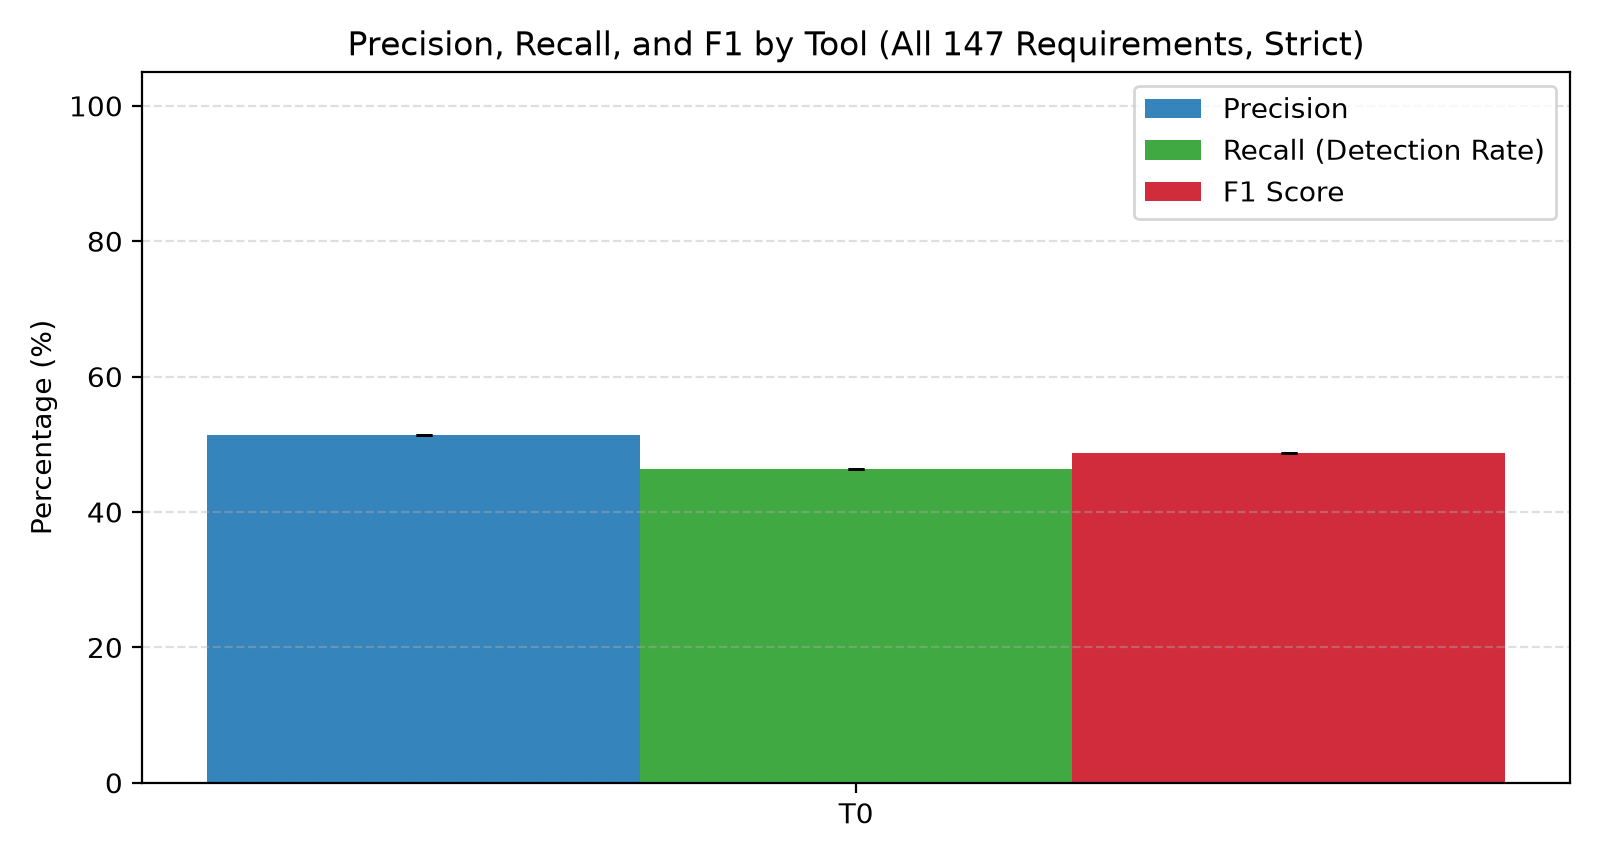
\includegraphics[height=0.66\textheight]{prf1_by_tool.png}\\[0.1cm]
  {\small Người rà soát đọc \numEffortTone{} cảnh báo/khiếm khuyết với T1, chỉ \numEffortTfour{} với T4. Mọi công cụ đều vượt mốc ``gắn cờ tất cả'' ($F_1$ \numFFlagAll\%).}
  \note{[Khánh] Cột cam là Recall, gần chạm 100 với mọi công cụ LLM. Cột xanh dương là Precision, thấp. Đường nét đứt là F1 khi gắn cờ mọi yêu cầu, khoảng 28 phần trăm; mọi công cụ đều cao hơn, nghĩa là chúng có chọn lọc thật. Về thực tế: với T1, người rà soát đọc khoảng 4 cảnh báo mới gặp một lỗi; với T4 chỉ khoảng 2,5.}
\end{frame}

% --- Slide 14: Skill effect ---
\begin{frame}{Tác động của kỹ năng \texttt{SKILL.md} (RQ2)}
  \begin{columns}[c]
    \begin{column}{0.55\textwidth}
      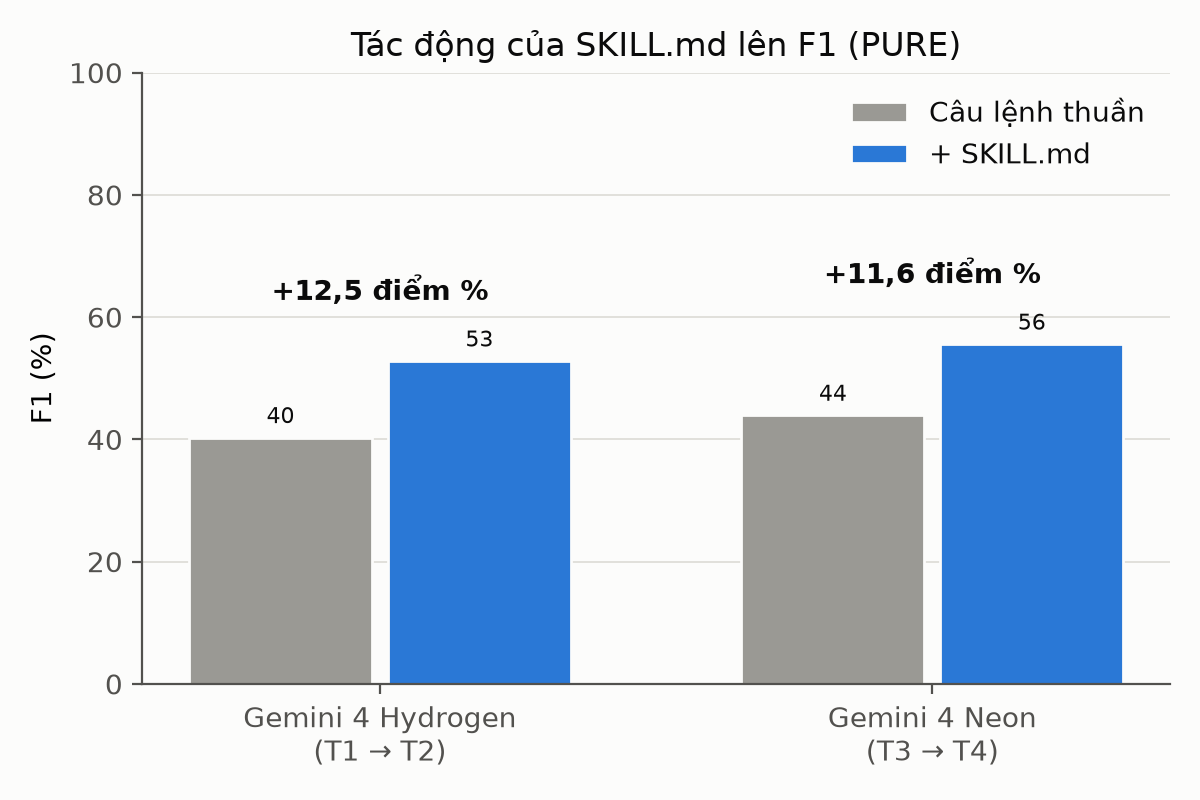
\includegraphics[width=\textwidth]{skill_effect.png}
    \end{column}
    \begin{column}{0.43\textwidth}
      \begin{itemize}\small
        \item Hydrogen: $\Delta F_1 = +\numSkillDFHydro$ điểm (KTC 95\%: \numSkillLoHydro--\numSkillHiHydro)
        \item Neon: $\Delta F_1 = +\numSkillDFNeon$ điểm (KTC 95\%: \numSkillLoNeon--\numSkillHiNeon)
        \item Nhờ \textbf{Precision} tăng khoảng 11 điểm, Recall chỉ giảm 5--6 điểm
        \item Neon chỉ hơn Hydrogen $+$\numModelDFPlain{} / $+$\numModelDFSkill{} điểm, nhưng chậm gấp 2 lần
        \item \textbf{Kỹ năng quan trọng hơn chọn mô hình}
      \end{itemize}
    \end{column}
  \end{columns}
  \note{[Nam] Kỹ năng tăng F1 khoảng 12 điểm ở cả hai mô hình, và khoảng tin cậy không chứa 0 nên có ý nghĩa thống kê. Lợi ích đến từ việc bớt cảnh báo yếu: Precision tăng khoảng 11 điểm, Recall chỉ giảm 5 đến 6 điểm. So sánh hai mô hình: Neon chỉ hơn Hydrogen 3 đến 4 điểm và chạy chậm gấp đôi. Vậy trang bị kỹ năng quan trọng hơn chọn mô hình.}
\end{frame}

% --- Slide 15: By defect type ---
\begin{frame}{Loại khiếm khuyết nào khó nhất? (RQ3)}
  \begin{columns}[T]
    \begin{column}{0.5\textwidth}
      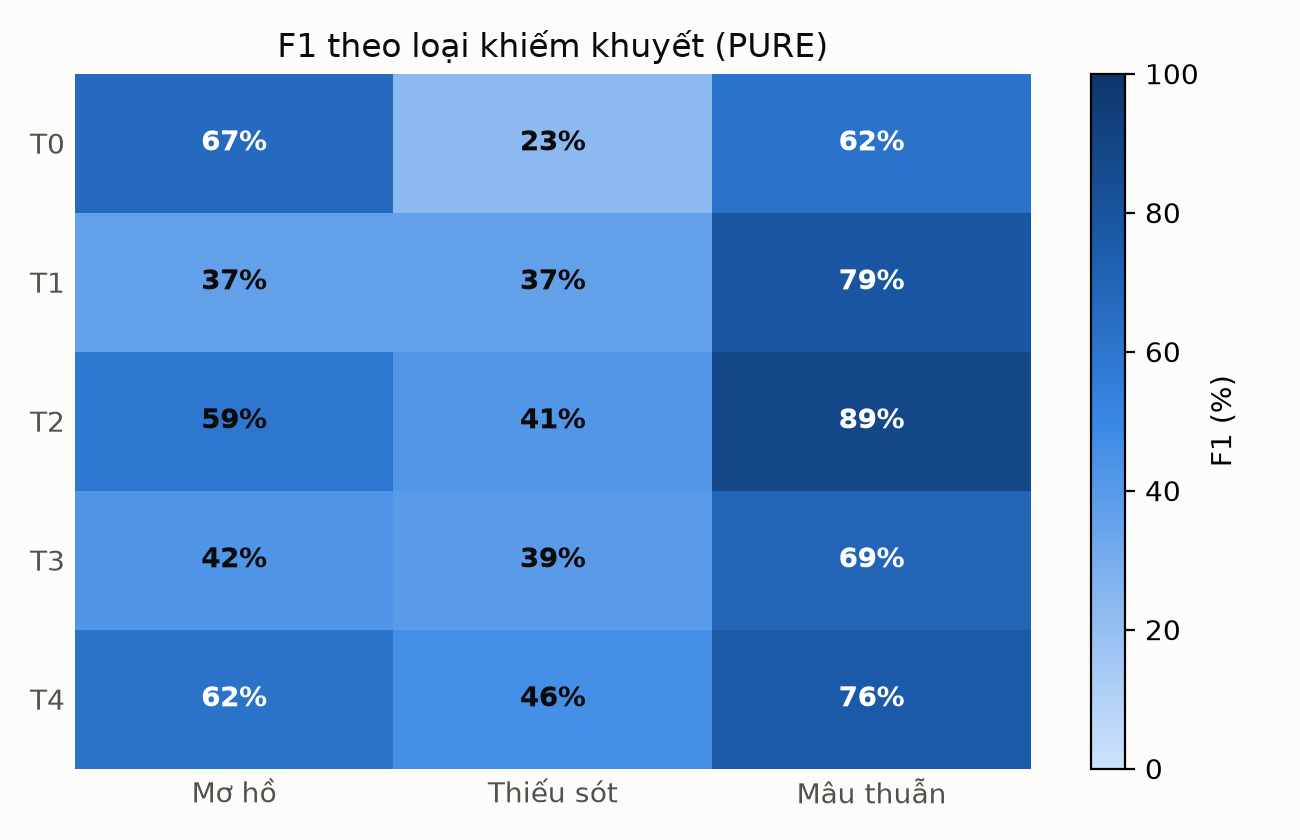
\includegraphics[width=\textwidth]{f1_heatmap.png}
    \end{column}
    \begin{column}{0.48\textwidth}
      \begin{itemize}\small
        \item \textbf{Mâu thuẫn dễ nhất:} $F_1$ \numFConTthree--\numFConTtwo\%
        \item \textbf{Thiếu sót khó nhất:} $F_1$ \numFIncTone--\numFIncTfour\% (T0: \numFIncTzero\%). Ranh giới giữa ``thiếu thật'' và ``có thể bổ sung'' mang tính phán đoán
        \item \textbf{Mơ hồ:} kỹ năng giúp nhiều nhất (\numFAmbTone\% $\rightarrow$ \numFAmbTtwo\%); bộ dò từ khóa T0 đã đạt \numFAmbTzero\%
        \item Recall của LLM $\ge$ 91\% ở mọi loại, nên khác biệt nằm ở Precision
      \end{itemize}
    \end{column}
  \end{columns}
  \note{[Nam] Bản đồ nhiệt thể hiện F1 theo loại lỗi. Mâu thuẫn và trùng lặp là dễ nhất. Thiếu sót là khó nhất, vì ranh giới giữa thiếu thông tin thật và có thể bổ sung thêm chi tiết mang tính phán đoán. Với lỗi mơ hồ, bộ dò từ khóa T0 đã làm rất tốt, nên có thể dùng T0 như bước lọc nhanh.}
\end{frame}

% --- Slide 16: Stability, sanity check, cost ---
\begin{frame}{Độ ổn định, kiểm tra hợp lý và chi phí (RQ4)}
  \begin{columns}[T]
    \begin{column}{0.5\textwidth}
      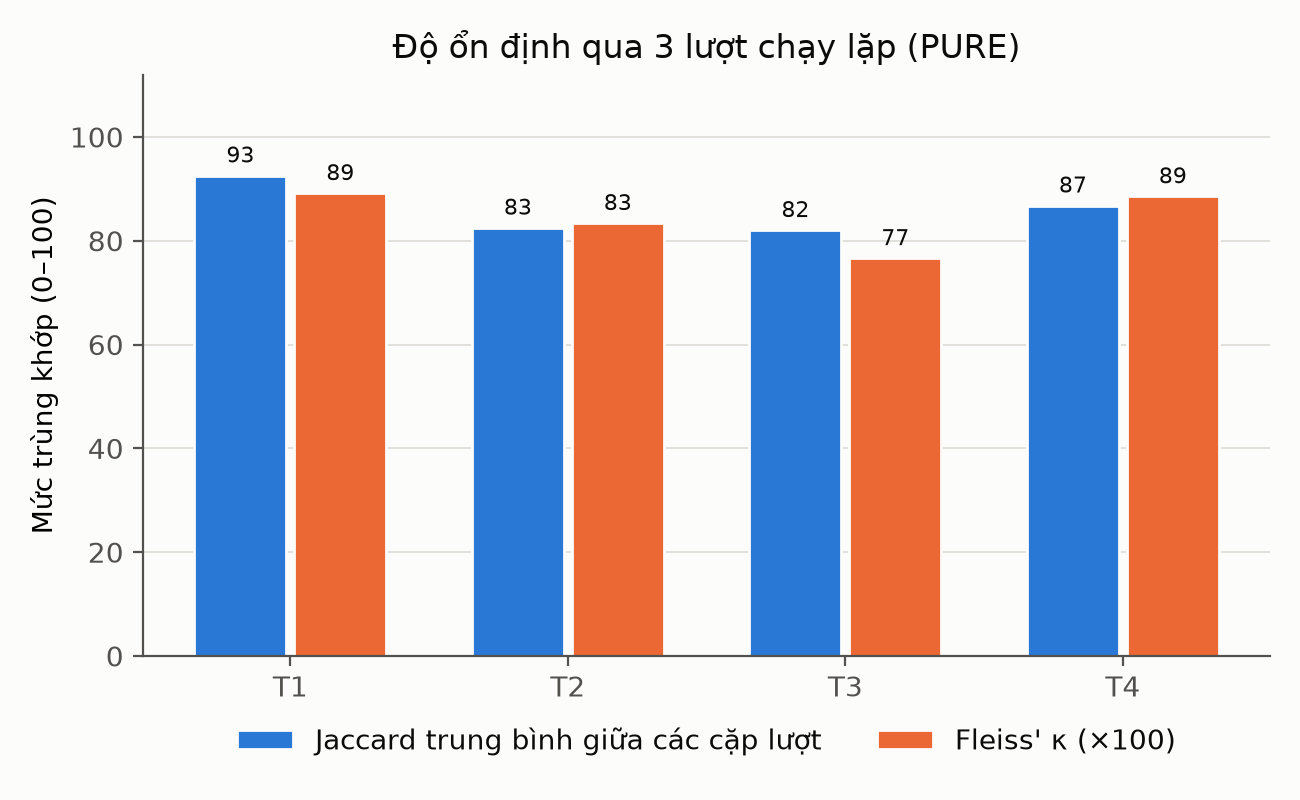
\includegraphics[width=\textwidth]{stability.png}
    \end{column}
    \begin{column}{0.48\textwidth}
      \begin{itemize}\small
        \item \textbf{Ổn định cao:} Jaccard \numJacTtwo--\numJacTone, Fleiss' $\kappa$ \numFleissTthree--\numFleissTone{} qua 3 lượt
        \item \textbf{Tài liệu cấy lỗi:} mọi LLM đạt $F_1$ \numFSeedTone--\numFSeedTfour\% $\Rightarrow$ chỉ dùng để kiểm tra hợp lý
        \item \textbf{Chi phí:} 48 lượt, \numAgyMinutes{} phút, \numAgyMTokens{} triệu token; \numDurTone{} giây/lượt (Hydrogen), \numDurTthree{} giây/lượt (Neon)
      \end{itemize}
    \end{column}
  \end{columns}
  \note{[Nam] Kết quả rất ổn định giữa 3 lượt chạy, Jaccard từ 0,82 đến 0,93, nên kết luận không phụ thuộc vào một lượt may rủi. Trên tài liệu cấy lỗi, mọi LLM đều gần 100 phần trăm: lỗi theo mẫu sách giáo khoa quá dễ, nên tài liệu này chỉ để kiểm tra hợp lý. Toàn bộ thực nghiệm tốn khoảng 2 giờ và 1,8 triệu token.}
\end{frame}

% --- Slide 17: Error analysis ---
\begin{frame}{Vì sao Precision thấp? Phân tích lỗi}
  \begin{columns}[T]
    \begin{column}{0.46\textwidth}
      \begin{block}{30 trường hợp bất đồng (ẩn nguồn)}
        \small
        \begin{itemize}
          \item Người rà soát AI: \numAIRevReal/\numAIRevN{} cảnh báo thừa là \textbf{lỗi thật}, \numAIRevBorder{} ở ranh giới
          \item $\Rightarrow$ khoảng \numAIRevRealLo--\numAIRevRealHi\% cảnh báo thừa có thể là lỗi thật bị nhãn chuẩn bỏ qua
          \item \numHCSlideC
        \end{itemize}
      \end{block}
    \end{column}
    \begin{column}{0.51\textwidth}
      \scriptsize
      \begin{exampleblock}{Lỗi thật nhãn chuẩn bỏ qua (\texttt{PE-004}, 12/12 lượt gắn cờ)}
        ``Resource provisioning, delegation and reservation policies are in place'': không nêu chính sách nào.
      \end{exampleblock}
      \begin{alertblock}{Đòi hỏi quá mức (\texttt{GJ-013})}
        ``The system shall be able to retrieve 200 products per second'': bị coi là \texttt{weak\_phrase} dù đã có con số.
      \end{alertblock}
      \begin{alertblock}{Không phải yêu cầu (\texttt{GJ-005})}
        Cụm ``easy of use'' nằm trong câu giải thích, không nằm trong yêu cầu.
      \end{alertblock}
    \end{column}
  \end{columns}
  \note{[Dương] Câu hỏi quan trọng: các cảnh báo thừa là nhiễu hay lỗi thật? Nhóm lấy 30 trường hợp bất đồng và ẩn nguồn khi đánh giá. Khoảng một phần ba đến một nửa cảnh báo thừa thực chất là lỗi thật mà nhãn chuẩn bỏ qua, ví dụ PE-004 không nêu chính sách nào. Cảnh báo sai chủ yếu do đòi hỏi quá mức, hoặc do công cụ gắn cờ ghi chú không phải yêu cầu. Nghĩa là Precision thật của công cụ cao hơn con số trong bảng.}
\end{frame}

% --- Slide 18: Limitations ---
\begin{frame}{Hạn chế và mối đe dọa tính hợp lệ}
  \begin{itemize}
    \item \textbf{Nhãn chuẩn do AI tạo:} giảm thiểu bằng 2 lượt độc lập, $\kappa$, kiểm định cấy lỗi, người rà soát thứ hai và kiểm tra bởi người. Nhãn chuẩn khá khắt khe nên Precision báo cáo là cận dưới.
    \item \textbf{Chỉ 2 mô hình Gemini:} kết luận chắc chắn cho họ mô hình này; tác động kỹ năng lặp lại ở cả hai mô hình.
    \item \textbf{Tài liệu cấy lỗi quá dễ:} PURE là thước đo chính.
    \item \textbf{Rò rỉ đáp án đã phát hiện và sửa:} ví dụ trong \texttt{SKILL.md}, luật T0, số lượng lỗi trong \texttt{seeded\_lms}; lượt chạy bị ảnh hưởng đã được chạy lại.
    \item \textbf{Quy mô nhỏ (107 yêu cầu thật):} có KTC bootstrap 95\%; PURE có thể đã nằm trong dữ liệu huấn luyện của LLM.
  \end{itemize}
  \note{[Dương] Nhóm nêu thẳng các hạn chế: nhãn chuẩn do AI tạo, nhưng đã có nhiều lớp kiểm tra, kể cả kiểm tra bởi người. Chỉ có hai mô hình Gemini, nên kết luận gắn với họ mô hình này. Trong quá trình làm, nhóm phát hiện và sửa ba chỗ rò rỉ đáp án; các lượt chạy bị ảnh hưởng đã được chạy lại.}
\end{frame}

% --- Slide 19: Conclusion & Q&A ---
\begin{frame}{Kết luận \& Hỏi đáp}
  \begin{block}{Trả lời 4 câu hỏi nghiên cứu}
    \begin{itemize}\small
      \item \textbf{RQ1:} LLM gần như không bỏ sót (Recall $\ge$ \numRTfour\%) nhưng Precision thấp (\numPTone--\numPTfour\%); $F_1$ tốt nhất \numFTfour\% (T4)
      \item \textbf{RQ2:} kỹ năng tăng $F_1$ khoảng 12 điểm ở cả hai mô hình, có ý nghĩa thống kê
      \item \textbf{RQ3:} thiếu sót khó nhất, mâu thuẫn dễ nhất
      \item \textbf{RQ4:} ổn định cao qua các lượt chạy (Jaccard $\ge$ \numJacTtwo)
    \end{itemize}
    \textbf{Khuyến nghị:} dùng LLM có kỹ năng làm \textbf{trợ lý sàng lọc} (AI đề xuất, người quyết định), kết hợp bộ dò luật để lọc nhanh.
  \end{block}
  \centering
  \vspace{0.2cm}
  {\Large\bfseries\color{hustred} Cảm ơn thầy và các bạn đã lắng nghe!}\\[0.1cm]
  {\small Mời thầy và các bạn đặt câu hỏi.}
  \note{[Dương] Tóm lại: LLM gần như không bỏ sót nhưng gắn cờ quá nhiều; kỹ năng là cách rẻ và hiệu quả để giảm nhiễu; thiếu sót là loại khó nhất; kết quả ổn định. Khuyến nghị dùng LLM có kỹ năng như trợ lý sàng lọc, con người là người quyết định cuối cùng. Cảm ơn thầy và các bạn, nhóm xin nhận câu hỏi.}
\end{frame}

% --- Slide 20: Live-demo backup slide (real T4 output) ---
\begin{frame}{Phụ lục: Demo dự phòng (đầu ra thật của T4)}
  \begin{columns}[T]
    \begin{column}{0.4\textwidth}
      \begin{block}{Đầu vào (\texttt{peering.json})}
        \ttfamily\scriptsize
        \{"req\_id": "PE-004",\\
        \hspace*{1em}"text": "Resource provisioning, delegation and reservation policies are in place"\}
      \end{block}
    \end{column}
    \begin{column}{0.57\textwidth}
      \begin{block}{Đầu ra (\texttt{result/run/T4/peering/run\_1.json})}
        \ttfamily\scriptsize
        \{"req\_id": "PE-004",\\
        \hspace*{1em}"type": "incompleteness",\\
        \hspace*{1em}"subtype": "missing\_actor",\\
        \hspace*{1em}"evidence": "are in place",\\
        \hspace*{1em}"related\_ids": [],\\
        \hspace*{1em}"rationale": "Omits which actor or system component defines, manages, and enforces the resource provisioning, delegation, and reservation policies, as well as the concrete policy rules."\}
      \end{block}
    \end{column}
  \end{columns}
  \note{[Dương] Slide dự phòng nếu demo trực tiếp lỗi: đây là đầu ra thật của T4 (Neon + kỹ năng) cho yêu cầu PE-004, đúng lược đồ JSON của kỹ năng.}
\end{frame}

\end{document}
